\documentclass[../functional-analysis_17-18.tex]{subfiles}

%Sample lecture



\begin{document}
	\section{Лекция 1. Метрические пространства.}
	
	\subsection{Метрические пространства.}
	
	Рассмотрим произвольное непустое множество $X$ и функцию $\rho\colon X \times X \to [0, +\infty)$.
	\begin{definition}
		Упорядоченная пара $(X, \rho)$  называется \textit{метрическим пространством}, если выполняются следующие свойства:
		\begin{enumerate}
			\item $\forall x \ \forall y: \rho(x, y) = 0 \iff x = y$
			\item $\forall x \ \forall y: \rho(x, y) = \rho(y, x)$
			\item $\forall x \ \forall y \ \forall z: \rho(x, y) \leq \rho(x, z) + \rho(z, y)$ (неравенство треугольника)
		\end{enumerate}
		В таком случае функция $\rho$ называется \textit{метрикой}.
	\end{definition}
	
	В общем случае, метрику нужно понимать как расстояние, так как мы от нее требуем истинность неравенство.0.0
	
	Посмотрим на некоторые примеры метрических пространств.
	
	\begin{enumerate}
		\item $\R,\ \rho(x, y) = |x - y|$
		
		Это обычное пространство со стандартным расстоянием.
		
		\item $\displaystyle \R^2, \ \rho(x, y) = \sqrt{(x_1 - y_1)^2 + (x_2 - y_2)^2}$
		
		Как говорится, так вас учила Марьиванна.
		
		\item $\displaystyle \R^n, \ \rho(x, y) = \sqrt{\sum_{i = 1}^n (x_i - y_i)^2}$
		
		Просто обобщаем пространство до $n$-мерного.
		
		\item $\displaystyle \{0, 1\}^n, \ \rho(x, y) = \sum_{i = 0}^n |x_i - y_i|$
	\end{enumerate}
	
	Последний пример называется \textit{булевым кубом} и играет большую роль в теории информации. В этом пространстве удобно строить так называемые \textit{коды Хэмминга}. Но для их рассмотрения нам нужно ввести еще несколько определений.
	
	\begin{definition}
		\textit{Открытым шаром} $B(a, r)$ с центром в точке $a$ и радиуса $r$ называется множество
		\begin{equation}
			B(a, r) = \{x: \ \rho(x, a) < r\}
		\end{equation}		
	\end{definition}
		\begin{definition}
		\textit{Замкнутым шаром} $B(a, r)$ с центром в точке $a$ и радиуса $r$ называется множество
		\begin{equation}
		\overline{B}(a, r) = \{x: \ \rho(x, a) \leq r\}
		\end{equation}		
	\end{definition}

	Здесь нужно обратить внимание на то, что шар в метрических пространствах может вести себя контринтуитивно, так как всю радость здесь дает метрика. Рассмотрим метрическое пространство $(\R^2, \ \rho(x, y))$, причем
	\begin{equation}
		\rho(x, y) = 
		\begin{cases}
			0, &x = y \\
			1, &\text{иначе}
		\end{cases}
		\textit{ -- дискретная метрика.}
	\end{equation}
	
	Тогда если взять произвольную точку $A$, то $\R^2 = B(A, 2)$. Иными словами, вся плоскость в такой метрике будет лежать в открытом шаре радиуса 2. При этом, $\{A\} = B(A, 1)$.
	
	\begin{wrapfigure}{r}{0.5\textwidth}
		\centering
		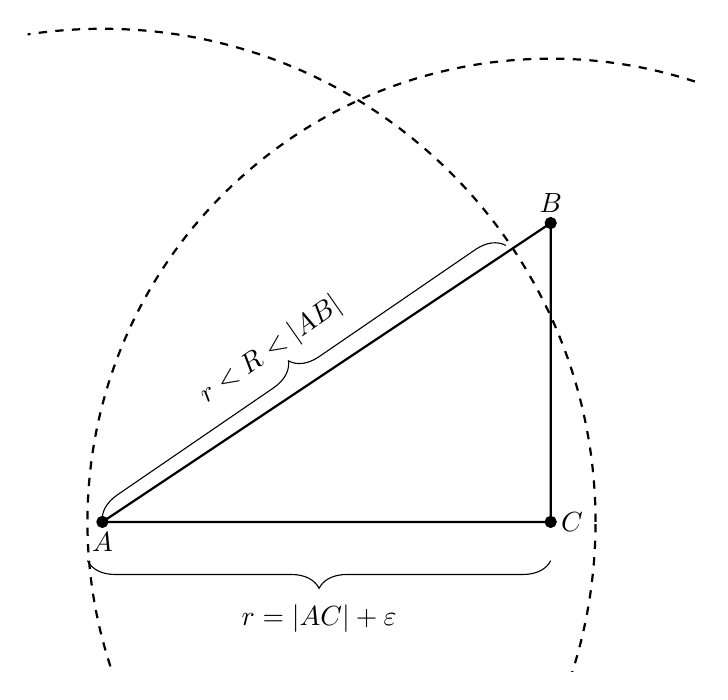
\begin{tikzpicture}
		\begin{axis}[
		scale=1.5,
		xmax=1,ymax=3.5, ymin=-1, xmin=-3.5,
		axis lines = none,
		axis equal image,
		]
		\draw[black,dashed, thick] (0, 0) circle(3.1);f
		\draw[black,dashed, thick] (-3, 0) circle(3.3);
		\draw [decorate,decoration={brace,amplitude=10pt, mirror,raise=4pt},xshift=0pt,yshift=-10pt]
		(-3.1, 0) -- (-0,0) node [black,midway, yshift=-25pt] 
		{$r=|AC|+\varepsilon$};
		\draw [decorate,decoration={brace,amplitude=10pt}]
		(-3, 0) -- (-0.3,1.85) node [black,midway, xshift=-12pt, yshift=12pt, rotate=35] 
		{$r<R<|AB|$};
		\draw[black, solid, thick]
		(-3,0) node[black, anchor=north]{$A$}
		-- (0,0) node[black, anchor=west]{$C$}
		-- (0, 2) node[black, anchor=south]{$B$}
		-- cycle;
		\addplot[only marks, black] coordinates {(0, 0) (0, 2) (-3, 0)};
		%			
		\end{axis}
		\end{tikzpicture}
	\end{wrapfigure}
	Рассмотрим пример, когда шар большего радиуса лежит внутри шара с меньшим радиусом (само собой, их центры не совпадают).
	
	Задано трехточечное пространство, где элементы расположены на плоскости, как показано на рисунке, то есть формируя прямоугольный треугольник $\triangle ABC$ с прямым углом при вершине $C$, и $|AB|>|BC|$. Возьмем шар $B(C, r)$, где $r$ больше $|AB|$ на малую величину $\varepsilon>0$, чтобы точка $A$ попала в открытый шар. Можно видеть, что шаром является все пространство. Теперь берем шар $B(A, R)$, где радиус $R>r$, но меньше длины гипотенузы (как известно, в любом прямоугольном треугольнике гипотенуза длиннее любого катета). Таким образом, из соотношения $|AC|=r-\varepsilon<r<R<|AB|$ следует, что в данном шаре лежат точки $A$ и $C$, но не $B$. 
	Таким образом, $B(A, R)\subset B(C, r)$, при  $R>r$.
	
	\subsection{Коды Хэмминга}
	Теперь мы можем перейти к кодам Хемминга.
	
%	\begin{wrapfigure}{r}{0.6\textwidth}
%		\centering
%		\begin{tikzpicture}
%		\begin{axis}[
%		scale=1.2,
%		xmax=3,ymax=4, ymin=-4, xmin=-3,
%		axis lines = none,
%		axis equal image
%		]
%		
%		
%		\draw[black, solid, thick]
%		(-3,0) node[black, anchor=north]{$A$}
%		-- (0,0) node[black, anchor=west]{$C$}
%		-- (0, 2) node[black, anchor=south]{$B$}
%		-- cycle;
%		\addplot[only marks, black] coordinates {(0, 0) (0, 2) (-3, 0)};
%		%			
%		\end{axis}
%		\end{tikzpicture}
%	\end{wrapfigure}
	Идея в том, что мы хотим создать такое кодирование, которое могло бы исправить нам одну ошибку. Посмотрим на булев куб размерности 3. В таком кубе есть вершины с координатами $(1, 1, 1)$ и $(0, 0, 0)$. Пусть $a = (0, 0, 0)$ и $b = (1, 1, 1)$. Такой куб разбивается на объединение $\overline{B}(a, 1) \cup \overline{B}(b, 1)$ при пустом пересечении. Тогда мы можем точно знать, что если пришли биты $000, 001, 010, 100$, то хотели передать бит $0$.  
	
	Нужно отметить, что в кубе не всякой размерности можно построить такой код. Во время такого построения мы разбиваем куб на $N$ шаров, в каждом у нас должно быть $n + 1$ вершина, где $n$ -- размерность куба. Но тогда
	
	\begin{equation}
		\begin{aligned}
			2^n &= (n + 1)N \\
			n &= \frac{2^n}{N} - 1
		\end{aligned}
	\end{equation}
	
	Так как размерность должна быть натуральным числом, количество шаров обязано быть степенью двойки, а значит размерность $n$ должна выражаться как
	
	\[
		n = 2^m - 1, m \in \N
	\]
	
	
	\TODO{Битовое представление}
	
	
	Есть интересная задача на коды Хэмминга, имеющая нетривиальное решение.
	\begin{task}
		В тюрьме в разных камерах сидят двое заключенных. Перед началом игры они могут выработать стратегию. Надзиратель на каждую клетку шахматной доски ставит монету произвольной стороной вверх. Он зовет в комнату первого заключенного и переворачивает на доске одну монеты. Заключенный может перевернуть ровно одну монету. Затем он покидает комнату и туда приходит второй заключенный. Его цель -- взглянув на доску указать монету, которая была изначально перевернута.
	\end{task}
	
	\subsection{p-адическая норма}
	\subsubsection{Определение}
	Понятие метрики индуцирует расстояние между точками множества, но так как метрика может быть произвольной, расстояние может выглядеть совершенно по-разному. Примером необычного расстояния может служить $p$-адическая норма.
	
	Работаем в $\Z$, фиксируем $p$ -- простое число. Возьмем произвольное $a \in \Z$, и представим его в виде
	\begin{equation}
		a = p^k \cdot a',
	\end{equation}
	где $GCD(p, a') = 1$. Иными словами, мы вытаскиваем из нашего числа максимальную степень $p$. 
	
	\begin{definition}
		\textit{$p$-адической нормой} числа $a$, обозначаемой как $\|a\|_p$ называется число
		\begin{equation}
			\|a\|_p = \frac{1}{p^k}
		\end{equation}		
	\end{definition}
	
	Естественным образом можно продолжить определение на $\Q$:
	\begin{equation}
		\left\|\frac{a}{b}\right\|_p = \frac{\|a\|_p}{\|b\|_p}
	\end{equation}
	
	\begin{statement}
		$\|\cdot\|_p$ -- \textit{нормирование}, то есть
		\begin{enumerate}
			\item $\forall x \ \|x\|_p \geq 0$, причем $\|x\|_p = 0 \iff x = 0$
			\item $\|xy\|_p = \|x\|_p\|y\|_p$
			\item $\|x + y\|_p \leq \|x\|_p + \|y\|_p$
		\end{enumerate}
	\end{statement}
	\begin{proof}
		Проверим, что все свойства выполняются.
		\begin{enumerate}
			\item Очевидно.
			\item Пусть $x = p^kx'$, $y=p^ly'$. Ну тогда верна цепочка равенств:
			\begin{equation}
				\|xy\|_p = \|p^kx' \cdot p^ly'\|_p = \|p^{k+l}\underbrace{(x'y')}_{\text{GCD=1}}\|_p = p^{k+l}x'y' = \|x\|_p\|y\|_p
			\end{equation}
			
			\item В этом пункте мы докажем более сильное утверждение, из которого будет вытекать наше, а именно, что
			\begin{equation}
				\|x+y\|_p \leq \max(\|x\|_p, \|y\|_p)
			\end{equation}
			
			Пусть $x = p^kx'$, $y=p^ly'$. Будем считать, что $k \geq l$. Тогда
			\begin{equation}
				x + y = p^kx' + p^ly' = p^l(p^{k - l}x' + y')
			\end{equation}
			
			Мы вытащили из суммы максимальную степень $p$, а значит
			\begin{equation}
				\|x + y\|_p \leq \frac{1}{p^l} = \max(\|x\|_p, \|y\|_p)
			\end{equation}
		\end{enumerate}
	\end{proof}
	\begin{corollary}
		$p$-адическая норма индуцирует метрику на $\Q$: $\rho(x, y) = \|x - y\|_p$.
	\end{corollary}
	\begin{proof}
		Первые два свойства метрики получаются автоматически, осталось только третье:
		\begin{equation}
			\|x - y\|_p = \|x - z + z - y\|_p \leq \|x - z\|_p + \|z - y\|_p
		\end{equation}
	\end{proof}
	
	\subsubsection{Чудеса}
	
	$p$-адическая норма творит чудеса на уже знакомых нам пространствах. Сейчас работам в $\Z$.
	
	\begin{enumerate}
		\item $\Z \subset \overline{B}(0, 1)$.
		
		Действительно, область значений нашей метрики лежит в отрезке $[0, 1]$.
		
		\item Пусть $B = B(a, r)$, для произвольных центра и радиуса. Пусть $c \in B$. Тогда верно, что
		\begin{equation}
			B(a, z) = B(c, r)
		\end{equation}
		\begin{proof}
			Докажем следующий факт, из которого вытекает наш:
			\begin{equation}
				x \in B(c, r) \then x \in B(a, r)
			\end{equation}
			
			Этот факт достается нам практически бесплатно:
			\begin{equation}
				\|x - a\|_p \leq \max(\underbrace{\|x - c\|_p}_{\leq r},\underbrace{\|xc - a\|_p}_{\leq r})
			\end{equation}
		\end{proof}
	\end{enumerate}
	
	\TODO{Близость к 1}
	
	
	\subsection{Сходимости}
	
	Понятие сходимости достаточно естественно для анализа и было бы просто замечательно описывать сходимость метрикой.
	
	\begin{definition}		
		Пусть $(X, \rho)$ -- метрическое пространство. Говорят, что последовательность $\{x_n\}$ сходится к $x$ \textit{по метрике} (также говорят, что сходимость \textit{задана метрикой}), если выполнено следующее:
		\begin{equation}
			x_n \underset{n \to \infty}{\longrightarrow}x \iff \rho(x_n, x) \underset{n \to \infty}{\longrightarrow}0
		\end{equation}
	\end{definition}
	
	Например, в $\R^2$ сходимость последовательности точек $(x_n, y_n) \to (x, y)$  равносильна покоординатной сходимости:
	\begin{equation}
		(x_n, y_n) \to (x, y) \iff x_n \to x \text{ и } y_n \to y
	\end{equation}
	
	Такую сходимость можно задать разными метриками, например $\rho(x, y) = \displaystyle \sqrt{(y_1 - x_1)^2 + (y_2 - x_2)^2}$, или $\rho(x, y) = \max(|y_1 - x_1|, |y_2 - x_2|)$. 
	
	Печальный факт состоит в том, что не все сходимости можно задать метрикой. Типичный пример: поточечная сходимость функций, определенных на отрезке $[0, 1]$. Напомним ее определение.
	
	\begin{definition}
		Последовательность функций $\{f_n\}$ сходится \textit{поточечно} к $f$, если
		\begin{equation}
			\forall t \in [0, 1]:  f_n(t) \underset{\text{как числовая}}{\longrightarrow} f(t)
		\end{equation}
	\end{definition}

	\begin{statement}
		Поточечная сходимость не может быть задана метрикой.
	\end{statement}
	\begin{proof}
		Докажем от противного. Пусть $\rho$ --  задающая поточечную сходимость метрика.
		Пусть $\Delta$ обозначает некоторый отрезок внутри $[0, 1]$. Пусть $I_\Delta$ --  индикатор этого отрезка.
		
		Возьмем шар $B(0, 1)$. Верно следующее утверждение:
		\begin{equation}
			\exists \Delta \subset (0, 1): |\Delta| > 0 \text{ и } I_\Delta \in B(0, 1)
		\end{equation}
		
		Построим последовательность отрезков $\Delta_i$, такую что $|\Delta| \to 0$, никакие два отрезка не пересекаются и для двух последовательных отрезков правый конец предыдущего меньше левого конца следующего и ни у какого отрезка правый конец не равен 1.
		
		\TODO{Рисуонк}
		
		Тогда на нашей последовательности отрезков последовательность функций-индиакторов поточечно сойдется к 0.
		
		Теперь начнем сжимать наши шары, беря все меньший и меньший радиус.
		
        \begin{equation}
			\begin{aligned}
				\exists N_1& \forall n > N_1: f_n \in B(0, 1) \\
				\exists N_2& \forall n > N_2: f_n \in B\left(0, \frac{1}{2}\right) \\
				\exists N_3& \forall n > N_3: f_n \in B\left(0, \frac{1}{3}\right) \\
				&\vdots\\
				\exists N_k& \forall n > N_k: f_n \in B\left(0, \frac{1}{k}\right)
			\end{aligned}
		\end{equation}
		
        Получим последовательность индикаторов. Для нее выполнено, что
        \begin{equation}
            \rho\left( I_{\Delta_n}, 0 \right) \leq \frac{1}{n}
        \end{equation}
        
        А значит, наша последовательность сойдется к тождественно нулевой функции. При этом наши шары обеспечили систему вложенных отрезков, а значит и общую точку, на которой индиактор равен 1. Противоречие.
	\end{proof}
	
    \subsection{Критерий Коши. Полное пространство}
    
    Для обсуждения полных пространств нам нужно вспомнить критерий Коши.
    
    \begin{definition}
        В метрическом пространстве последовательность $\{x_n\}$ сходится к  предельной точке $x$ \textit{по Коши} (удовлетворяет критерию Коши), если   
        \begin{equation}
            \forall \epsilon > 0 \ \exists N \in \N \ \forall n, m > N \ \rho(x_n, x_m) \leq \epsilon
        \end{equation}
        
    \end{definition}
    
    \begin{definition}
        Пространство $(X, \rho)$ называется \textit{полным}, если в нем выполняется критерий Коши.
    \end{definition}
	
    Простейший пример не полного метрического пространства это $(\R \setminus \{a\}, |\cdot|)$ -- выкинули из прямой одну точку. Тогда можно указать последовательность, для которой выполняется критерий Коши, в $\R$ она сходится к точке $a$,  но в нашем множестве ее предельная точка выкинута.                                                 
    
    \begin{theorem}
        Если $(X, \rho)$ -- полное метрическое пространство и задана последовательность вложенных замкнутых шаров $\overline{B}_{r_1} \supset \ldots \supset \overline{B}_{r_n} \supset \ldots $, причем $r_n \underset{n \to \infty}{\longrightarrow} 0$, то их пересечение непусто и состоит из одной точки
        \begin{equation}
            \bigcap_n \overline{B}_{r_n} = \{c\}
        \end{equation}
    \end{theorem}
	\begin{proof}
        Для начала разберемся с единственностью, так как она получается почти автоматически.
        
        Пусть в пересечении лежали две точки $c_1$  и  $c_2$. Дальше осталось заметить, что
        \begin{equation}
            \rho(c_1, c_2) \leq 2r_n \underset{n \to \infty}{\longrightarrow} 0 \then \rho(c_1, c_2) \to 0
        \end{equation}
        
        Осталось существование, что является менее очевидным фактом.
        
        Построим последовательность точек $\{x_n\}$, такую что $\forall n \ x_n \in \overline{B}_{r_n}$. Заметим, что для такой последовательности выполняется критерий Коши. Зафиксируем $N \in \N$ и положим $n, m > N$.
        Так как $ \overline{B}_{r_N} \supset \overline{B}_{r_n} $ и $ \overline{B}_{r_N} \supset \overline{B}_{r_m} $ можем заключить, что 
        \begin{equation}
            \rho(x_n, x_m) \leq 2r_N \leq \epsilon
        \end{equation}
        
        Значит у нашей последовательности есть предельная точка $x_0$. Покажем, что она лежит в пересечении, то есть лежит в каждом шаре. Для этого заметим, что 
        \begin{equation}
            \left| \rho(x_n, a) - \rho(x_0, a) \right| \leq \rho(x_n, x_0)
        \end{equation}
        где $a$ -- центр шара радиуса $r_n$.
    \end{proof}
	
	
	
	
	
	
	
	
	
\end{document}